\documentclass[tikz]{standalone}
\usepackage{tikz}
\usepackage[AutoFakeBold=true,AutoFakeSlant=true]{xeCJK}
\usepackage[zihao=-4,UTF8,heading=true]{ctex}
\usepackage[simplified]{pgf-umlcd}
\usetikzlibrary{fit} %形状
\usetikzlibrary{positioning} %不加方向运算可能出错
\usetikzlibrary{arrows.meta} %箭头
\usetikzlibrary{calc}

\setCJKmainfont{微软雅黑}
\begin{document}
	\thispagestyle{empty}
    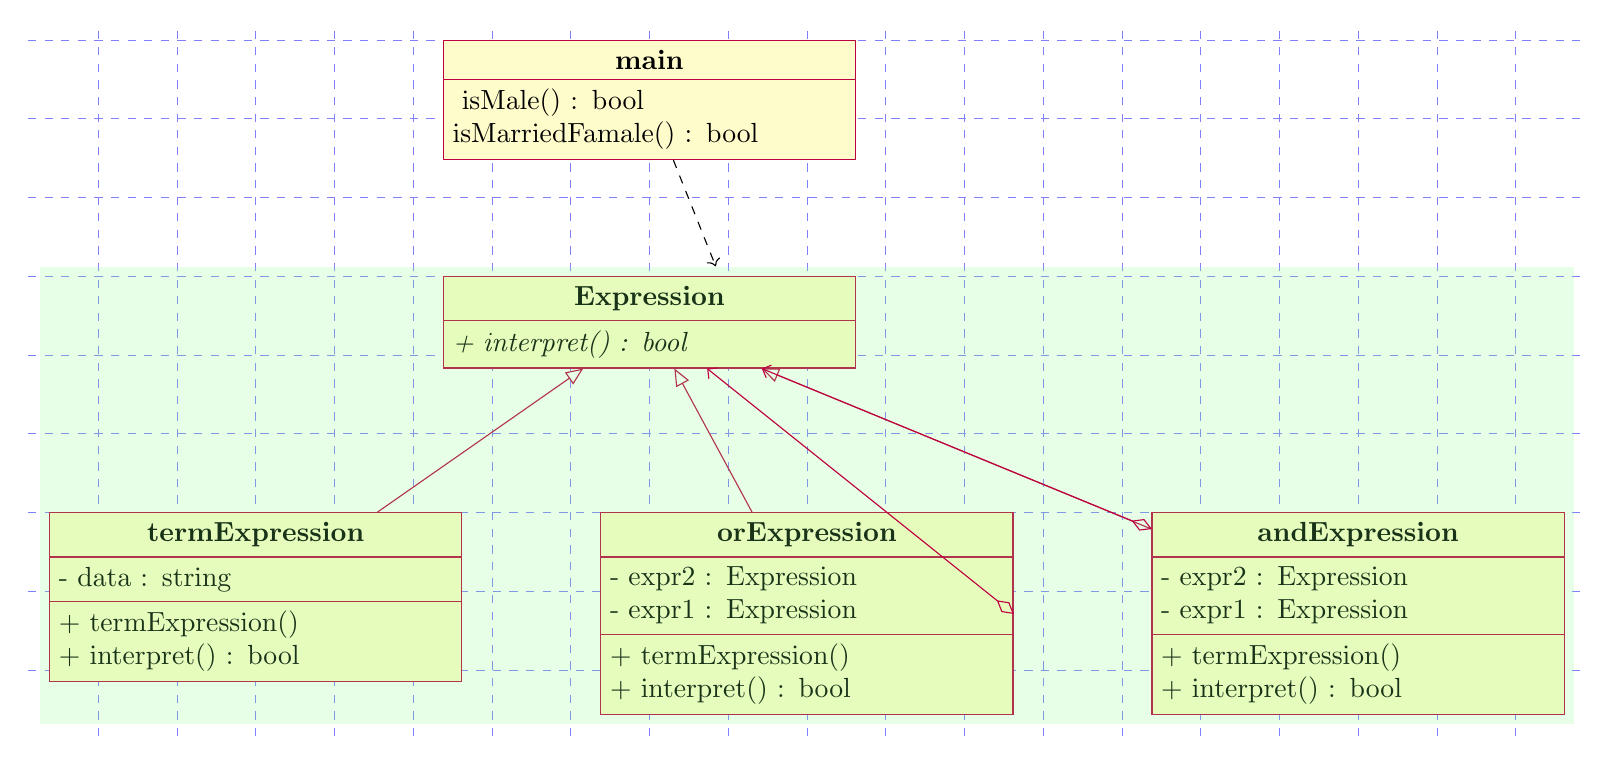
\begin{tikzpicture}[show background grid]
        \begin{class}[text width=5cm]{Expression}{0,0}
            \operation[0]{+ interpret() : bool}
        \end{class}
        \begin{class}[]{termExpression}{-5, -3}
            \attribute{- data : string}
            \inherit{Expression}
            \operation{+ termExpression() }
            \operation{+ interpret() : bool}
        \end{class}
        \begin{class}[]{orExpression}{2, -3}
            \inherit{Expression}
            \attribute{- expr2 : Expression }
            \attribute{- expr1 : Expression }
            \operation{+ termExpression() }
            \operation{+ interpret() : bool}
        \end{class}
        \begin{class}[]{andExpression}{9, -3}
            \inherit{Expression}
            \attribute{- expr2 : Expression }
            \attribute{- expr1 : Expression }
            \operation{+ termExpression() }
            \operation{+ interpret() : bool}
        \end{class}
        \node[fill=green!50,fill opacity=.2,
        fit=(Expression)(termExpression)
        (orExpression)(andExpression)](Expr){};

        \begin{class}[]{main}{0, 3}
            \attribute{ isMale() :  bool}
            \attribute{ isMarriedFamale() : bool }
        \end{class}
        \draw [dashed, ->] (main) -- (Expr);
        \aggregation{orExpression.east}{}{}{Expression}
        \aggregation{andExpression}{}{}{Expression}
    \end{tikzpicture}

\end{document}